

\newpage
\section{Experiments}
Following tests performed by applying 10-fold cross-validation, averaged over 10 different randomized runs. Moreover, in order to decrease computational requirements, the number of Naive Bayes classifiers in the bagging ensemble is restricted to 10. In each experiment, results of the new approach are compared with cost-sensitivity (see~\ref{costsensitive}), MetaCost (see~\ref{MetaCost}) and Bagging for Imbalanced datasets (see~\ref{BaggingImbalanced}).

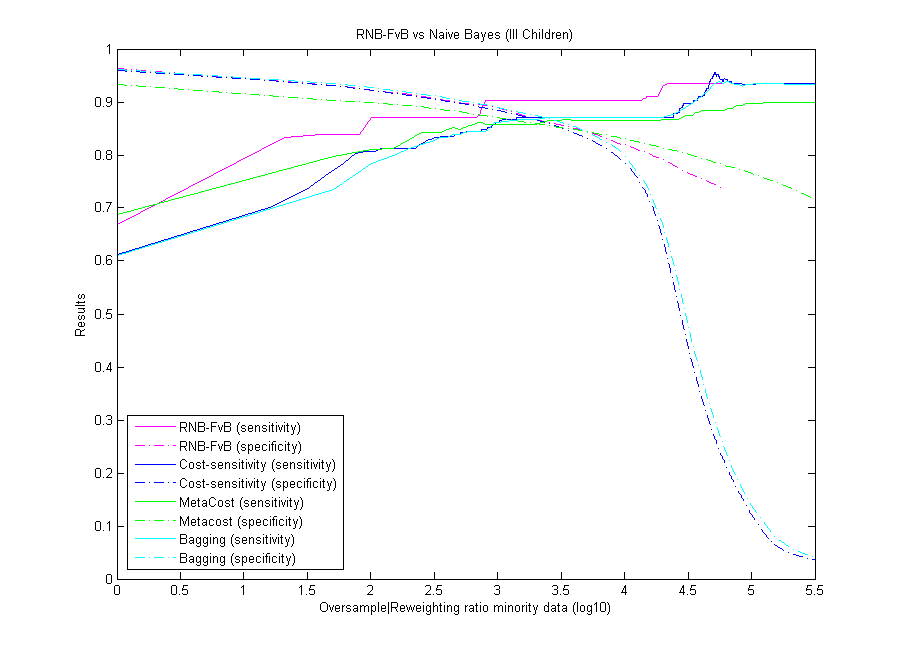
\includegraphics[scale=0.65]{img/RNB-FvB-illchildren.png}
 
\begin{table}[h]
\centering  
\begin{tabular}{ l | c r | r r|}                                      
& \multicolumn{2}{c}{max AUC (sample ratio)} & \multicolumn{2}{c}{max sensitivity (specificity)} \\
\hline 
RNB-FvB & 0.9479 & (x\,60\,000) & 93.55\% & (78.61\%)\\
Cost-sensitivity & 0.9040 & (x\,1) & 95.48\% & (26.95\%)\\
MetaCost & 0.9206 & (x\,1) & 100.00\% & (12.54\%)\\
Bagging & 0.9128 & (x\,1) & 86.45\% & (87.05\%)\\
\hline                          % inserts single-line
\end{tabular}
\label{tab:PPer}
\caption{Overview Results RNB-FvB for Ill Children} % title name of the table
\end{table}
 




\newpage
Since it is important to measure the performance of a new technique in many datasets in order to allow generalisation of results, the same tests were performed on some UCI datasets (\url{http://archive.ics.uci.edu/ml/}) and averaged over 10 randomized runs:\\\\
\textbf{Breast-cancer}: the breast cancer domain was obtained from the University Medical Centre, Institute of Oncology, Ljubljana, Yugoslavia (1988). Thanks go to M. Zwitter and M. Soklic for providing the data. The data set includes 85 instances of one class (\textit{recurrence-events}) and 201 instances of another class (\textit{no-recurrence-events}). The instances are described by 9 attributes, of which all are nominal. In the following graph, performance results of Random Naive Bayes with Feature-value bootstrapping is compared with regular Naive Bayes (reweighting the \textit{recurrence-events} class).

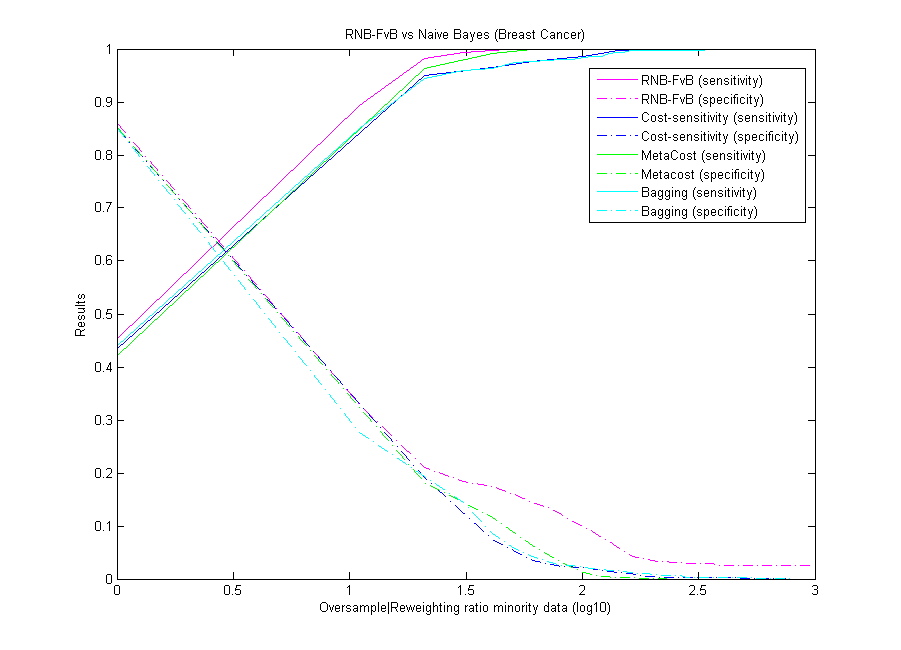
\includegraphics[scale=0.65]{img/RNB-FvB-breastcancer.png}

\begin{table}[h]
\centering  
\begin{tabular}{ l | c r | r r|}                                      
& \multicolumn{2}{c}{max AUC (sample ratio)} & \multicolumn{2}{c}{max sensitivity (specificity)} \\
\hline 
RNB-FvB & 0.7450 & (x\,271) & 100.00\% & (15.92\%)\\
Cost-sensitivity & 0.6981 & (x\,1) & 100.00\% & (0.30\%)\\
MetaCost & 0.7187 & (x\,41) & 100.00\% & (3.03\%)\\
Bagging & 0.6951 & (x\,1) & 95.65\% & (15.87\%)\\
\hline                          % inserts single-line
\end{tabular}
\label{tab:PPer}
\caption{Overview Results RNB-FvB for Breast-cancer} % title name of the table
\end{table}


\newpage
\textbf{Hepatitis}: the hepatitis domain was donated by G. Gong, Carnegie-Mellon University, Ljubljana, Yugoslavia (1988). The data set includes 32 instances of one class (\textit{die}) and 123 instances of another class (\textit{live}). The instances are described by 19 attributes, of which 6 are numeric and 13 are nominal. In the following graph, performance results of Random Naive Bayes with Feature-value bootstrapping is compared with regular Naive Bayes (reweighting the \textit{die} class).
 
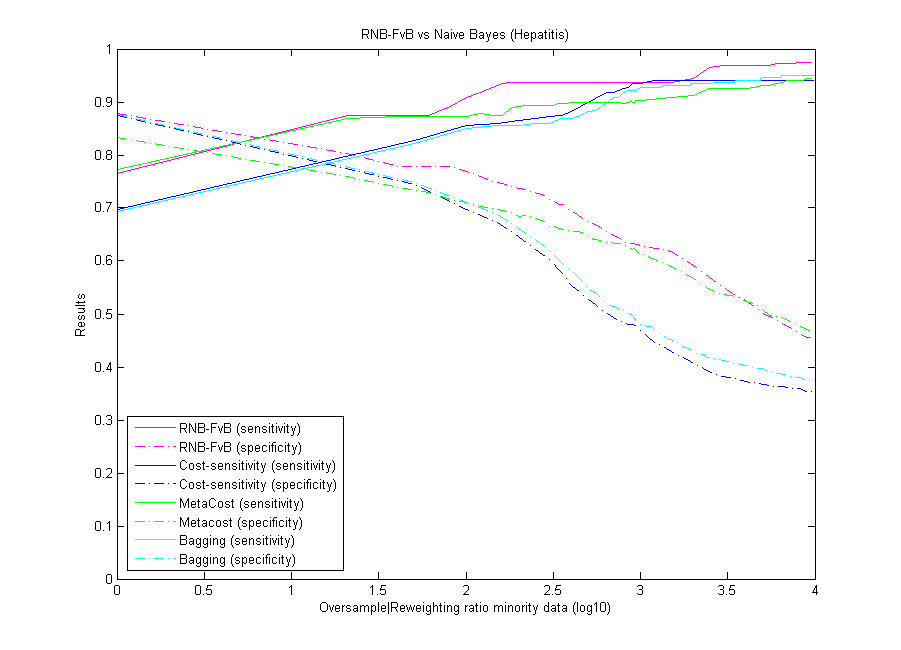
\includegraphics[scale=0.65]{img/RNB-FvB-hepatitis.png}

\begin{table}[h]
\centering  
\begin{tabular}{ l | c r | r r|}                                      
& \multicolumn{2}{c}{max AUC (sample ratio)} & \multicolumn{2}{c}{max sensitivity (specificity)} \\
\hline 
RNB-FvB & 0.9101 & (x\,7\,500) & 97.50\% & (46.42\%)\\
Cost-sensitivity & 0.8639 & (x\,51) & 94.06\% & (44.72\%)\\
MetaCost & 0.8710 & (x\,21) & 94.37\% & (47.07\%)\\
Bagging & 0.8723 & (x\,1) & 95.31\% & (44.39\%)\\
\hline                          % inserts single-line
\end{tabular}
\label{tab:PPer}
\caption{Overview Results RNB-FvB for Hepatitis} % title name of the table
\end{table}

\newpage
\textbf{Sick}: this dataset conciders Thyroid disease records supplied by the Garavan Institute and the New South Wales Institute (J. Ross Quinlan), Sydney, Australia. The dataset includes 231 instances of one class (\textit{sick}) and 3541 instances of another class (\textit{negative}). The instances are described by 29 attributes, of which  7 are continuous and 23 are discrete. In the following graph, performance results of Random Naive Bayes with Feature-value bootstrapping is compared with regular Naive Bayes (reweighting the \textit{sick} class).

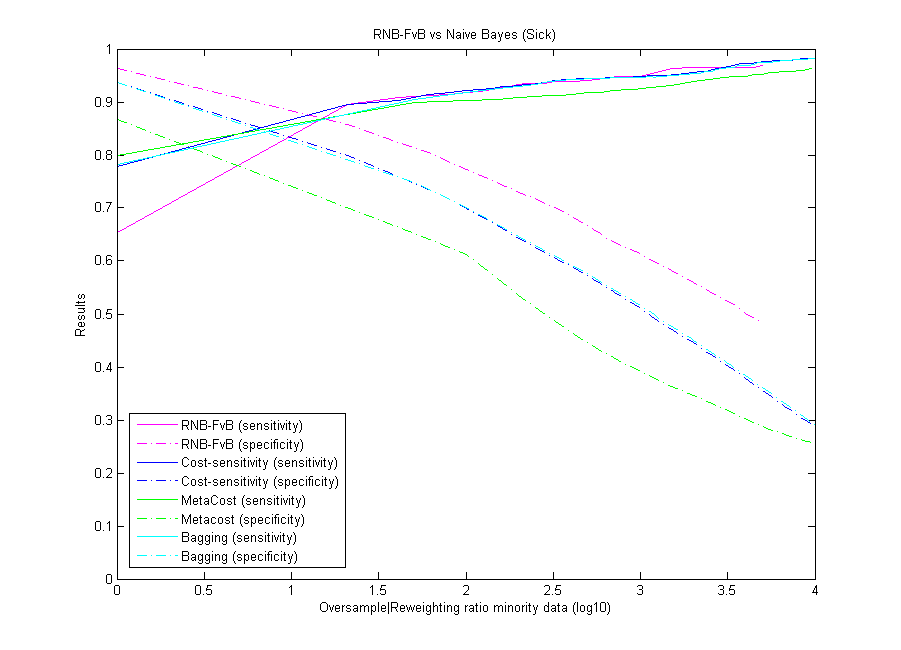
\includegraphics[scale=0.65]{img/RNB-FvB-sick.png}

\begin{table}[h]
\centering  
\begin{tabular}{ l | c r | r r|}                                      
& \multicolumn{2}{c}{max AUC (sample ratio)} & \multicolumn{2}{c}{max sensitivity (specificity)} \\
\hline 
RNB-FvB & 0.9322 & (x\,1) & 96.97\% & (48.18\%)\\
Cost-sensitivity & 0.9253 & (x\,1) & 98.23\% & (29.74\%)\\
MetaCost & 0.8898 & (x\,1) & 96.23\% & (25.73\%)\\
Bagging & 0.9281 & (x\,1) & 96.84\% & (36.92\%)\\
\hline                          % inserts single-line
\end{tabular}
\label{tab:PPer}
\caption{Overview Results RNB-FvB for Sick} % title name of the table
\end{table}

\newpage
\textbf{Liver-disorders}: This dataset contains blood tests (taken from male individuals) which are thought to be sensitive to liver disorders that might arise from excessive alcohol consumption. The dataset includes 145 instances of one class and 200 instances of another class. The instances are described by 6 attributes, of which all are continuous. In the following graph, performance results of Random Naive Bayes with Feature-value bootstrapping is compared with regular Naive Bayes where the minority data is reweighted.

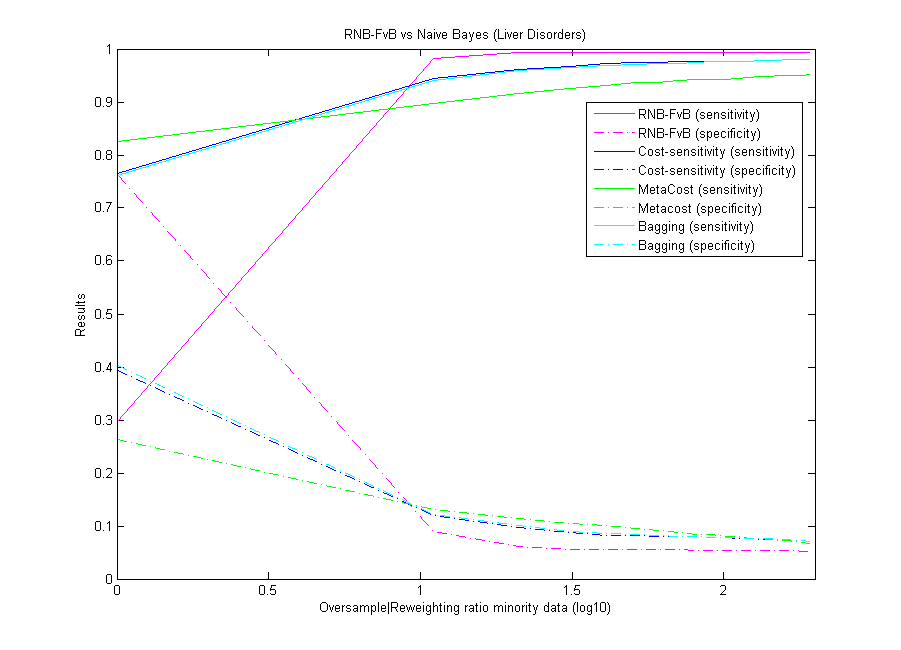
\includegraphics[scale=0.65]{img/RNB-FvB-liverdisorder.png}

\begin{table}[h]
\centering  
\begin{tabular}{ l | c r | r r|}                                      
& \multicolumn{2}{c}{max AUC (sample ratio)} & \multicolumn{2}{c}{max sensitivity (specificity)} \\
\hline 
RNB-FvB & 0.5744 & (x\,11) & 99.31\% & (6.05\%)\\
Cost-senstivity & 0.6331 & (x\,171) & 97.93\% & (7.25\%)\\
MetaCost & 0.5804 & (x\,11) & 95.10\% & (6.75\%)\\
Bagging & 0.6328 & (x\,161) & 98.00\% & (6.65\%)\\
\hline                 
\end{tabular}
\label{tab:PPer}
\caption{Overview Results RNB-FvB for Liver-disorders} 
\end{table}
Note that the lower AUC values for RNB-FvB are probably related to the fact that the used bootstrapping technique for continuous features is a mathematically not optimal solution. However, it is clear that RNB-FvB outperforms Naive Bayes even when all features are bootstrapped this way.
